\documentclass[compress]{beamer}

\usetheme{CambridgeUS}
\usecolortheme{rose}

\usepackage{amsmath,amsfonts,amssymb}
\usepackage{caption}
\usepackage{cancel}
\usepackage{enumerate}
\usepackage{graphicx}
\usepackage{floatrow}
\usepackage{hyperref}
\captionsetup[table]{labelformat=empty}
\newcommand{\expect}[1]{\mathbb{E} \left[ #1 \right]}
\newcommand{\expects}[2]{\mathbb{E}_{#1} \left[ #2 \right]}


\title{Variational Approaches for Auto-Encoding Generative Adversarial Networks}
\author[Presentor: Shih-Ming Wang]{Mihaela Rosca, Balaji Lakshminarayanan \\ David Warde-Farley, Shakir Mohamed}
\institute[]{Presented by Shih-Ming Wang \\ ComputerVision Lab, UCSC}
\date{02-13-2019}
\subject{Computer Science}
\graphicspath{{img/}}


\begin{document}

\begin{frame}
    \maketitle
    \hypertarget{titlePage}{}
\end{frame}

\begin{frame}
\frametitle{Authors}

\begin{columns}
    \begin{column}{.3\textwidth}
        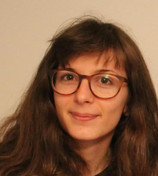
\includegraphics[width=\textwidth]{auth1} 
    \end{column}
    \begin{column}{.2\textwidth}
        \tiny
        \textbf{Mihaela Rosca} \\
        Research Engineer \\
        DeepMind \\
    \end{column}
    \begin{column}{.3\textwidth}
        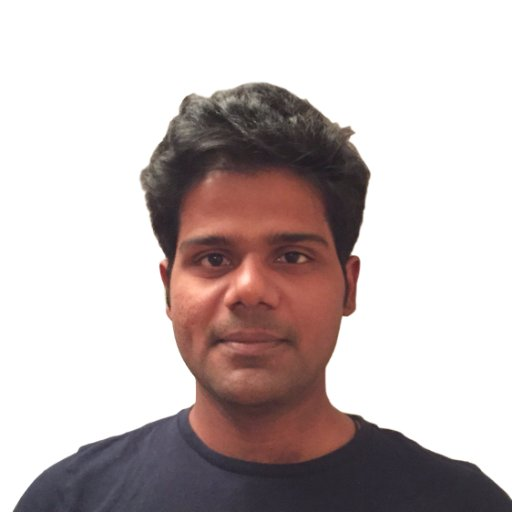
\includegraphics[width=\textwidth]{auth2} 
    \end{column}
    \begin{column}{.2\textwidth}
        \tiny
        \textbf{Balaji Lakshminarayanan} \\
        Senior Research Scientist \\
        DeepMind \\
    \end{column}
\end{columns}
\vfill
\begin{columns}
    \begin{column}{.3\textwidth}
        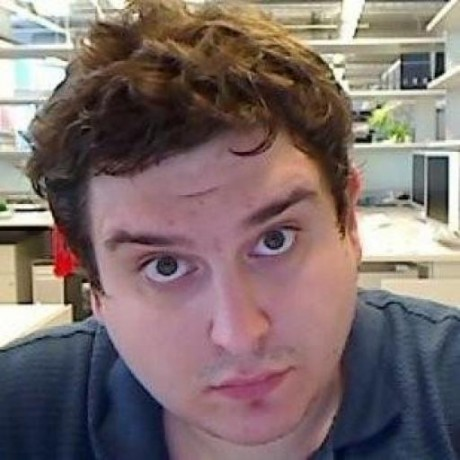
\includegraphics[width=\textwidth]{auth3} 
    \end{column}
    \begin{column}{.2\textwidth}
        \tiny
        \textbf{David Warde-Farley} \\
        Senior Research Scientist \\
        DeepMind \\
    \end{column}
    \begin{column}{.3\textwidth}
        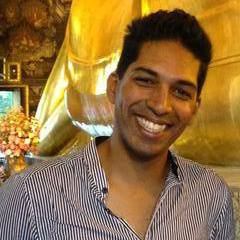
\includegraphics[width=\textwidth]{auth4} 
    \end{column}
    \begin{column}{.2\textwidth}
        \tiny
        \textbf{Shakir Mohamed} \\
        Research Scientist \\
        DeepMind \\
    \end{column}
\end{columns}

\end{frame}

\section{Motivation}
\begin{frame}[allowframebreaks]{Latent Variable Model}
    \begin{itemize}
        \item \textbf{Assumes} a generating process for real data $x\sim p^*(x)$
            \begin{itemize}
                \item Unobserved quantity following prior distribution $z\sim p_\theta(z)$
                \item Observation given $z$ following likelihood $x|z\sim p_{\theta}(x|z)$
            \end{itemize}
        \item Without losing generality, $z\sim \mathcal{N}(0, I)$ (dropping $\theta$ hereafter)
        \item Though $p_{\theta}(x,z)=p^*(x)p_{\theta}(z|x)$, it's not trivial to do inference (i.e. compute $p_{\theta}(z|x)$)
        \item Implicit Latent Variable Model, e.g. GAN
            \begin{itemize}
                \item Learns a generator $G_{\theta}$ and makes likelihood implicit: $p_{\theta}(x|z)= \delta(x-G_{\theta}(z))$
            \end{itemize}
        \item Prescribed Latent Variable Model, e.g. VAE
            \begin{itemize}
                \item \textbf{Assumes} explicit (closed form) likelihood $p_{\theta}(x|z)$
                \item \textbf{Assumes} explicit (closed form) posterior $p_{\theta}(z|x)$
                \item Approximates posterior $p_{\theta}(z|x)$ , hence able to do inference
            \end{itemize}
    \end{itemize} 
    \framebreak
    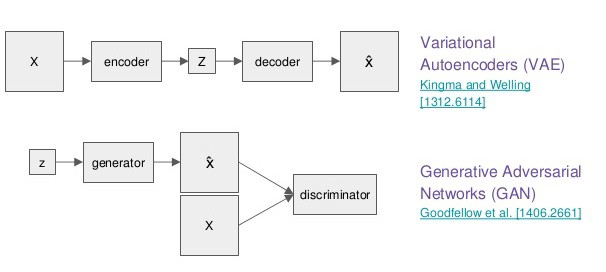
\includegraphics[height=.8\textheight,width=\textwidth]{vaeandgan}

\end{frame}

\begin{frame}{Motivation}
    \begin{block}{Generative Adversarial Network (GAN) Pros \& Cons}
        \begin{itemize}
            \item Excels at generating sharp samples
            \item Only make assumption on prior
            \item Optimization is hard (vanishing gradient) using its original loss
            \item The samples might lack diversity (mode-collapse)
            \item Can't do inference
        \end{itemize} 
    \end{block}  
    \begin{block}{Variational Auto Encoder (VAE) Pros \& Cons}
        \begin{itemize}
            \item Generates blurry images
            \item Requires assumption on likelihood posterior, limiting model power
            \item Pairwise reconstruction penalty discourages mode-collapse
            \item Can do inference
        \end{itemize}
    \end{block}
\end{frame}

\section{Background}
\begin{frame}{KL divergence}
    \begin{itemize}
        \item KL divergence measures ``distance'' between distributions
            \begin{align*}
                KL(p\|q) = \expects{p(x)}{\ln \frac{p(x)}{q(x)} } = \int p(x) \ln \frac{p(x)}{q(x)} dx 
            \end{align*}
        \item $KL(p\|q)\ge 0$, with equality hold when $p(x)=q(x), \forall x$
        \item Requirement to approximate $KL(p\|q)$
            \begin{itemize}
                \item Able to sample from $p(x)$
                \item $p(x), q(x)$ bare close form
            \end{itemize}
        \item In some cases, for e.g. when p, q are both Gaussian, $KL(p\|q)$ bares close form and sampling is not required
        \item KL is asymmetric, but Jenson-Shanon divergence (JSD) is
            \begin{equation*}
                JS(p\|q) = 0.5KL(p\|(p+q)/2) + 0.5KL(q\|(p+q)/2)
            \end{equation*}
    \end{itemize}
\end{frame}
\begin{frame}[t]{Jenson Inequality}
    \begin{itemize}
        \item For concave function $f$ and arbitrary distribution $p$
            \begin{align*}
                f(\expects{p(x)}{x})\ge \expects{p(x)}{f(x)}
            \end{align*}
        \item Which implies for any function $g$
            \begin{align*}
                f(\expects{p(x)}{g(x)})\ge \expects{p(x)}{f(g(x))}
            \end{align*}
        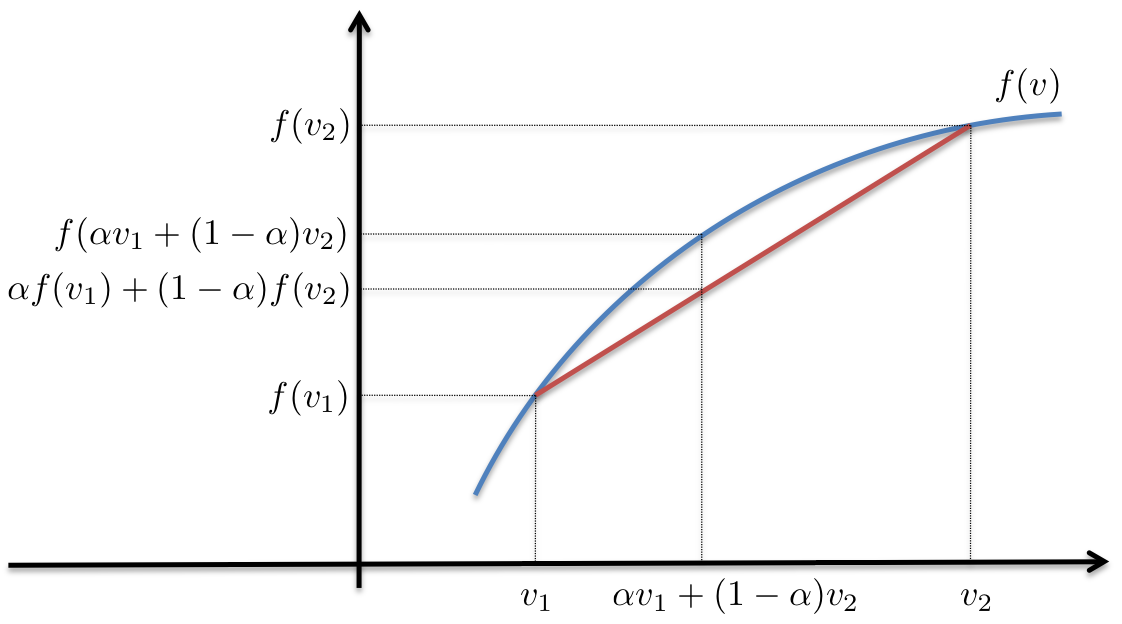
\includegraphics[height=.5\textheight]{jenson}
    \end{itemize}
\end{frame}

\begin{frame}[allowframebreaks]{Backpropagating through samples}
    \begin{itemize}
        \item Say we want to minimize $L(\theta, \eta) = \expects{p_{\eta}(x)}{f_{\theta}(x)}$
        \item Computing $\nabla_{\theta} L(\theta, \eta)$ is straightforward
            \begin{align*}
                \nabla_{\theta} L(\theta, \eta) & = \expects{p_\eta(x)}{\nabla_{\theta} L(\theta, \eta)} \\
                                                & \approx \frac{1}{n} \sum_{i=1}^n \nabla_\theta f_{\theta}(x_i), \forall x_i\sim p_{\eta}(x)
            \end{align*}
        \item However $\nabla_\eta L(\theta, \eta)$ is not in expectation form
            \begin{align*}
                \nabla_\eta L(\theta, \eta) & = \nabla_\eta \int p_\eta(x) f_\theta(x) dx \\
                                            & =  \int \nabla_\eta p_\eta(x) f_\theta(x) dx 
            \end{align*}
    \end{itemize}
    \framebreak
    \begin{block}{Score function estimator (REINFORCE)}
        \begin{itemize}
            \item  use the identity $\nabla_\eta p_\eta(x) = p_\eta(x) \nabla_\eta \log p_{\eta}(x)$
                \begin{align*}
                    \nabla_{\eta} L(\theta, \eta) & = \int \nabla_\eta p_\eta(x) f_\theta(x) dx \\
                                                  & = \int p_\eta(x)\nabla_\eta \log p_\eta(x) f_\theta(x) dx \\ 
                                                  & = \expects{p_\eta(x)}{f_\theta(x)\nabla_\eta \log p_\eta(x)} \\
                                                  & \approx \frac{1}{n} \sum_{i=1}^n f_\theta(x)\nabla_\eta \log p_\eta(x)
                \end{align*}
            \item Such estimator of the gradient might have high variance
        \end{itemize}
    \end{block}
    \framebreak
    \begin{block}{Reparameterization Trick}
        \begin{itemize}
            \item \textbf{Assume} 
                \begin{itemize}
                    \item $f_\theta(x)$ is differentiable w.r.t. $x$
                    \item Exists $g$, $x=g(\eta, \epsilon)$, where $\epsilon \sim p(\epsilon)$. 
                    \item For e.g. $x\sim \mathcal{N}(\mu(\eta)+\sigma^2(\eta))$ can be reparameterize as $x=\mu(\eta)+\sigma^2(\eta)*\epsilon, \epsilon\sim \mathcal{N}(0,1)$
                \end{itemize}
            \item Then we get an gradient estimator with low variance 
                \begin{align*}
                    \nabla_\eta L(\theta, \eta) & = \nabla_\eta \expects{p_\eta(x)}{f_\theta(x)} \\
                                                & = \nabla_\eta \expects{p(\epsilon)}{f_\theta(g(\eta, \epsilon))} \\
                                                & = \expects{p(\epsilon)}{\nabla_\eta f_\theta(g(\eta, \epsilon))} \\
                                                & = \expects{p(\epsilon)}{f'_\theta(g(\eta, \epsilon))\nabla_\eta g(\eta, \epsilon)} \\
                \end{align*}
        \end{itemize}
        
    \end{block}

\end{frame}

\begin{frame}{Maximum Log-Likelihood Principle (MLP)}
    \begin{itemize}
        \item MLP optimizes $\theta$ so that $p_{\theta}(x)\rightarrow p^*(x)$
            \begin{align*}
                \theta = \mathop{argmax}_{\theta} \frac{1}{n}\sum_{i=1}^n \ln p_{\theta}(x), \forall x_i \sim p^*(x)
            \end{align*}
        \item MLP is equivalent to minimizing KL divergence
            \begin{align*}
                \mathop{argmin}_{\theta} KL(p^*(x)\|p_{\theta}(x)) & = \mathop{argmin}_{\theta} E_{p^*(x)} \left[ \ln \frac{p^*(x)}{p_{\theta}(x)}  \right]
                 \\
                                                                   & = \mathop{argmin}_{\theta} E_{p^*(x)}[-\ln p_{\theta}(x)] + \cancel{\expects{p^*(x)}{\ln p^*(x)}}\\
                                                                   & \sim \mathop{argmax}_{\theta} \frac{1}{n}\sum_{i=1}^n \ln p_{\theta}(x_i), \forall x_i \sim p^*(x)
            \end{align*}
        \item Marginal likelihood is intractable (no closed form) in Latent Variable Model
            \begin{align*}
                p_{\theta}(x) = \int p(z)p_{\theta}(x|z) dz
            \end{align*}
    \end{itemize}
\end{frame}

\begin{frame}[t]{Choice of Loss}
    \begin{itemize}
        \item When MLP is intractable, different training objective are adopted
        \item Most objectives are consistent with MLP given infinite data and model capacity
        \item With limited model capacity, different objective can lead to very different result
        \item GAN approximately minimizes JSD, leading to mode-collapse
        \item VAE approximates MLP (minimizes KLD), leading to unreal sample
    \end{itemize}
    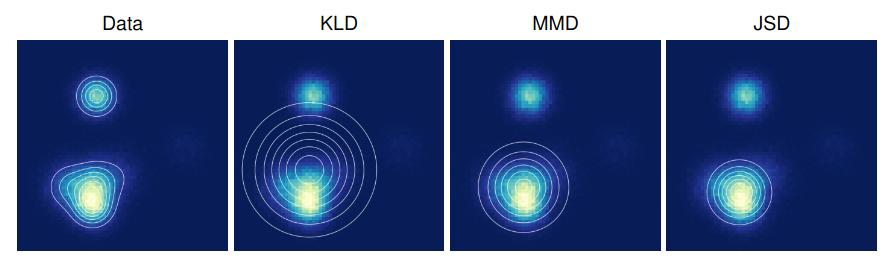
\includegraphics[height=0.4\textheight,width=\textwidth]{loss}
    \tiny{Figures from \cite{theis2015note}}
\end{frame}


\section{GANs \& VAEs}
\begin{frame}[allowframebreaks]{GAN}
        \begin{itemize}
            \item GAN estimates $ \frac{p^*(x)}{p_{\theta}(x)} $ with a discriminator $D_{\phi}$
            \item The input to the discriminator follows $0.5 p^*(x) + 0.5p_{\theta}(x)$
                \begin{align*}
                    \frac{p^*(x)}{p_{\theta}(x)} = \frac{p_\phi(x|y=1)}{p_\phi(x|y=0)} = \frac{\cancel{p(x)}p_\phi(y=1|x)/\cancelto{0.5}{p(y=1)}}{\cancel{p(x)}p_\phi(y=0|x)/\cancelto{0.5}{p(y=0)}} = \frac{D_{\phi}(x)}{1-D_{\phi}(x)}   
                \end{align*}
            \item The likelihood is $\prod_{i=1}^n D_{\phi}(x)^{y_i}(1-D_{\phi}(x))^{1-y_i}$, hence MLP for $\phi$ is
                \begin{align*}
                    \phi = \mathop{argmax}_{\phi}\expects{p^*(x)}{\ln D_{\phi}(x)} + \expects{p_{\theta}(x)}{\ln(1-D_{\phi}(x))}
                \end{align*}
            \item Fixing $D_\phi$, optimizes the following loss w.r.t. the generator $G_{\theta}$
                \begin{align*}
                    \theta = \mathop{argmin}_{\theta} \expects{p_\theta(x)}{\ln (1-D_{\phi}(x))}
                \end{align*}
        \end{itemize}

    \framebreak
    \begin{itemize}
        \item This is the minmax game that GAN played
            \begin{align*}
                & \mathop{min}_{\theta}\mathop{max}_{\phi} \expects{p^*(x)}{\ln D_{\phi}(x)} + \expects{p_{\theta}(x)}{\ln(1-D_{\phi}(x))} \\
                \leftrightarrow & \mathop{min}_{\theta}\mathop{max}_{\phi} \expects{p^*(x)}{\ln D_{\phi}(x)} + \expects{p(z)}{\ln(1-D_{\phi}(G_{\theta}(z)))}
            \end{align*}
        \item We need to be able to
            \begin{itemize}
                \item sample from implicit likelihood $p_\theta(x|z)$
            \end{itemize}
        \item We can do
            \begin{itemize}
                \item sample from model distribution $p_\theta(x)=p(z)p_\theta(x|z)$
            \end{itemize}
        \item We can't do
            \begin{itemize}
                \item compute $p_{\theta}(x)$ given $x$
                \item compute $p_{\theta}(z|x)$ or sample $z\sim p_{\theta}(z|x)$ given $x$
            \end{itemize}
    \end{itemize}
\end{frame}

\begin{frame}[allowframebreaks]{VAE}
    \begin{itemize}
        \item Variational Inference (VI) bounds $p_{\theta}(x)$ with evidence lower bound (ELBO) and follows MLP to maximize the ELBO:
            \begin{align*}
                \ln p_{\theta}(x) & = \ln \int p(z)p_{\theta}(x|z) dz & \\
                                  & =  \ln \int q_{\eta}(z) \frac{p(z)}{q_{\eta}(z)} p_{\theta}(x|z) dz & \\
                                  & =  \ln \expects{q_{\eta}(z)}{ \frac{p(z)}{q_{\eta}(z)} p_{\theta}(x|z)}&  \\
                                  & \ge \expects{q_{\eta}(z)}{ \ln \left(  \frac{p(z)}{q_{\eta}(z)} p_{\theta}(x|z)\right) } & \text{(Jenson Inequality)}\\
                                  & = \expects{q_{\eta}(z)}{ \ln \left(  \frac{p_{\theta}(x,z)}{q_{\eta}(z)} \right) } & (ELBO_1)\\
                                  & = \expects{q_{\eta}(z)}{\ln p_{\theta}(x|z)} + KL(q_{\eta}(z)\|p(z)) & (ELBO_2)
            \end{align*}
    \end{itemize}
    \framebreak
    \begin{itemize}
        \item $q_{\eta}(z)$ (variational distribution) serves as approximate posterior
        \item EM algorithm alternates between the two steps
            \begin{itemize}
                \item M-step: Fixing $q_{\eta}(z)$, optimize ELBO w.r.t. $\theta$ \\
                \item E-step: Fixing $p_{\theta}$, optimize ELBO w.r.t. $q_{\eta}(z)$
                    \begin{align*}
                        q_{\eta}(z) &  = \mathop{argmax}_{q_\eta(z)}\expects{q_{\eta}(z)}{ \ln \left(  \frac{p_{\theta}(x,z)}{q_{\eta}(z)} \right) } & (ELBO_1)\\
                                    &  = \mathop{argmax}_{q_\eta(z)}\expects{q_{\eta}(z)}{ \ln \left(  \frac{p(x)p_{\theta}(z|x)}{q_{\eta}(z)} \right) } & \\
                                    &  = \mathop{argmax}_{q_\eta(z)} \ln p(x) + \expects{q_{\eta}(z)}{ \ln \left(  \frac{p_{\theta}(z|x)}{q_{\eta}(z)} \right) } & \\
                                    &  =  \mathop{argmax}_{q_\eta(z)} \cancel{\ln p(x)} - KL(q_{\eta}(z)\|p_{\theta}(z|x)) & \\ 
                                    & = p_{\theta}(z|x) & \\
                    \end{align*}
            \end{itemize}
    \end{itemize}
    \framebreak
    \begin{itemize}
        \item $p_{\theta}(x)$ in $p_{\theta}(z|x)= \frac{p(z)p_{\theta}(x|z)}{p(x)} $ is usually intractable
        \item Usually assume parametric form $q_{\eta}(z)$ and optimize $\eta$ so that $q_{\eta}(z)\rightarrow p_\theta(z|x)$
        \item $q_\eta(z)$ usually has local parameters for each sample $x$. Alternatively, we can ``armortize'' it by modeling $q_\eta(z|x)$ with global parameters
    \end{itemize}
    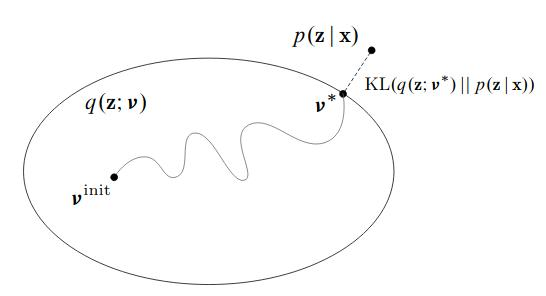
\includegraphics[scale=0.5]{vae}
    {
        \tiny{Figures from \cite{blei2016variational}}
    }
    \framebreak

    \begin{itemize}
        \item VAE models $q_{\eta}(z|x)$ with encoder $E_{\eta}$ and $p_{\theta}(x|z)$  with decoder $G_{\theta}$ 
        \item \textbf{Assumes} posterior $q_{\eta}(z|x_n) \sim \mathcal{N}(E_{\eta}(x_n), E_{\eta}(x_n) \mathbb{I})$
        \item \textbf{Assumes} likelihood $p_{\theta}(x_n|z) \sim \mathcal{N}(G_{\theta}(x_n), \mathbb{I})$
        \item Train $\eta, \theta$ simultaneously to minimizes $ELBO_2$
            \begin{align*}
                \eta, \theta = \mathop{argmax}_{\eta, \theta} \expects{q_{\eta}(z|x)}{\ln p_{\theta}(x|z)} + KL(q_{\eta}(z|x)\|p(z))
            \end{align*}
                
        \item VAE use reparameterization trick to estimate $\nabla_\eta \expects{q_{\eta}(z|x)}{\ln p_{\theta}(x|z)}$
        \item The first term is the reconstruction loss (auto-encoder)
        \item The second term serves a regularization, leading to higher reconstruction error
    \end{itemize}
    \framebreak
    \begin{itemize}
        \item This is the game that VAE played
            \begin{align*}
                \eta, \theta = \mathop{argmax}_{\eta, \theta} \expects{q_{\eta}(z|x)}{\ln p_{\theta}(x|z)} + KL(q_{\eta}(z|x)\|p(z))
            \end{align*}
        \item We need to be able to
            \begin{itemize}
                \item compute likelihood $p_\theta(x|z)$
                \item compute posterior approximation $q_{\eta}(z|x)$
            \end{itemize}
        \item We can do
            \begin{itemize}
                \item sample from model distribution $p_\theta(x)=p(z)p_\theta(x|z)$
                \item compute $q_{\theta}(z|x)$ or sample $z\sim q_{\theta}(z|x)$ given $x$
            \end{itemize}
        \item We can't do
            \begin{itemize}
                \item compute $p_{\theta}(x)$ given $x$
            \end{itemize}
    \end{itemize}
\end{frame}

\section{Fusion of VAE \& GAN}
\begin{frame}[t]{Fusion of VAE \& GAN}
    \begin{block}{Key Idea}
        \begin{itemize}
            \item Starts with VAE architecture
            \item Remove the close form assumption for $q_{\eta}(z|x)$ and $p_{\theta}(x|z)$ 
            \item Use implicit distribution for 
                \begin{itemize}
                    \item posterior: $q_{\eta}(z|x)=\delta(z-E_{\eta}(x))$
                    \item likelihood: $p_{\theta}(x|z)=\delta(x-G_{\theta}(z))$
                \end{itemize}
            \item Use the GAN trick to learn two discriminators $C_{\omega}$ and $D_{\phi}$ to estimate the two terms in ELBO
        \end{itemize}
    \end{block}
    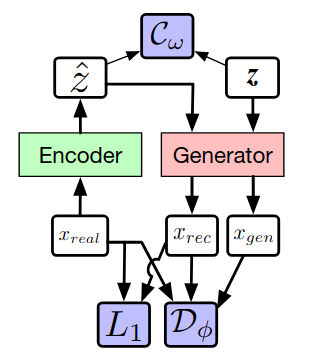
\includegraphics[scale=.3]{alphagan}
\end{frame}

\begin{frame}[t]{Implicit Variational Decomposition}
    \begin{itemize}
        \item Instead of Gaussian, let $q_{\theta}(z|x)=\delta(z-E_{\eta}(x))$ 
        \item The KL term in ELBO can be estimated by
            \begin{align*}
                KL(q_{\eta}(z|x)||p(z)) = \expects{q_{\eta}(z|x)}{\ln \frac{q_{\eta}(z|x)}{p(z)} } \approx \expects{q_{\eta}(z|x)}{\ln \frac{C_{\omega}(z)}{1-C_\omega(z)} }
            \end{align*}
        \item $C_{\omega}$ is a discriminator trained to tell samples drawn from $q_{\eta}(z|x)$ or $p(z)$
    \end{itemize}
\end{frame}

\begin{frame}[t]{Hybrid Likelihood}
    \begin{itemize}
        \item Let $p_{\theta}(x|z) = \delta(x-G_{\theta}(z))$
        \item The reconstruction term in ELBO can be estimated by
            \begin{align*}
                \expects{q_{\eta}(z|x)}{\ln p_{\theta}(x|z)} & = \expects{q_{\eta}(z|x)}{\ln \left( \frac{p_{\theta}(x|z)}{p^*(x)} p^*(x) \right)}   \\
                                                             & = \expects{q_{\eta}(z|x)}{\ln \frac{p_{\theta}(x|z)}{p^*(x)} } + \cancel{\ln p^*(x)}  \\
                                                             & \approx \expects{q_{\eta}(z|x)}{\ln \frac{D_\phi(G_{\theta}(z))}{1- D_\phi(G_{\theta}(z)) }}
            \end{align*}
        \item $D_{\phi}$ is a discriminator trained to tell samples from $p_{\theta}(x|z)$ or $p^*(x)$
        \item We can hybrid the implicit likelihood with an explicit likelihood 
        \item For e.g. Laplace: $p_\theta(x|z)\propto \exp(-\lambda\|x-G_{\theta}(z)\|_1)$, which leads to the $L_1$ reconstruction loss $\expects{q_{\eta}(z|x)}{-\lambda\|x-G_{\theta}(z)\|_1}$
    \end{itemize}
\end{frame}

\begin{frame}[allowframebreaks]{$\alpha$-GAN}
    \begin{itemize}
        \item This is the total loss of $\alpha-GAN$
            \begin{align*}
                \mathcal{L}(\theta, \eta) = \expects{q_{\eta}(z|x)}{-\lambda\|x-G_{\theta}(z)\|_1 + \ln \frac{D_\phi(G_{\theta}(z))}{1- D_\phi(G_{\theta}(z)) } + \ln \frac{C_{\omega}(z)}{1-C_\omega(z)}}
            \end{align*}
        \item The loss for $D_\phi$ and $C_{\omega}$ are not shown
        \item We need to be able to
            \begin{itemize}
                \item train encoder $E_{\eta}$, decoder $G_{\theta}$, and discriminators $D_{\phi}$, $C_\omega$
                \item sample from implicit posterior $z\sim q_{\eta}(z|x)$
                \item sample from implicit likelihood $x\sim p_{\theta}(x|z)$
                \item compute explicit likelihood $p_{\theta}(x|z)$
            \end{itemize}
        \item We can do
            \begin{itemize}
                \item sample from model distribution $p_\theta(x)=p(z)p_\theta(x|z)$
                \item sample from implicit posterior $q_{\theta}(z|x)$ given $x$
            \end{itemize}
        \item We can't do
            \begin{itemize}
                \item compute $p_{\theta}(x)$ given $x$
                \item compute $q_{\theta}(z|x)$ given $x$
            \end{itemize}
    \end{itemize}
    \framebreak
    \begin{block}{Tricks to improve}
        \begin{itemize}
            \item For the two discriminator, use a different loss to avoid vanishing gradient
            \item Pass reconstruct sample $x_{rec} \sim G_{\theta}(E_{\eta}(x))$ as well as sample from noise $x_{gen}\sim \sim G_{\theta}(z)$ to train $D_{\phi}$
        \end{itemize}
    \end{block}
    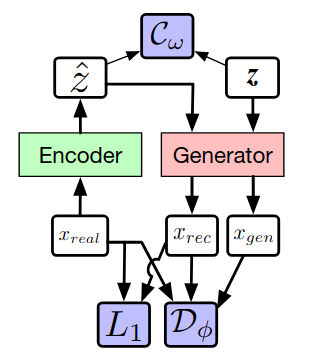
\includegraphics[scale=.4]{alphagan}
\end{frame}

\section{Related Work}
\begin{frame}[allowframebreaks]{Related Work}
    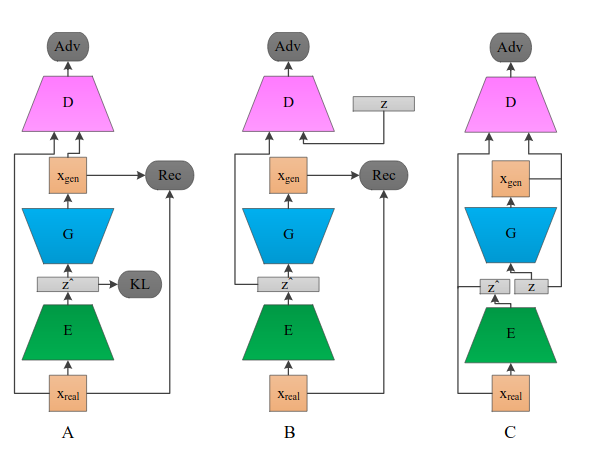
\includegraphics[scale=0.45]{relatedwork}
    {\tiny{Figures from \cite{huang2018introvae}}}
    \begin{enumerate}[A]
        \item VAEGAN imposes a discriminator $(D_\phi)$ on the data space
        \item AAE imposes a discriminator $(C_\omega)$ on the latent space
        \item ALI \& BiGan discriminate \textbf{jointly} in the data and latent space
    \end{enumerate}
    \framebreak
    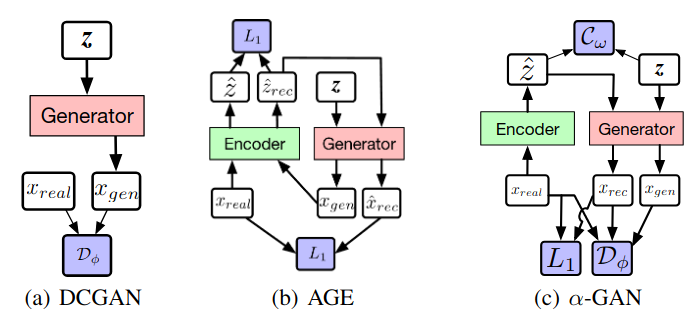
\includegraphics[scale=0.5]{relatedwork2}
    \begin{itemize}
        \item DCGAN is the normal GAN with some architecture tweaks
        \item AGE adds a \textbf{loop} from Generator back to Encoder, which is used as discriminator
        \item $\alpha-GAN$ imposes two discriminator on the data space and the latent space
    \end{itemize}
\end{frame}

\section{Evaluation}
\begin{frame}[t]{Evaluation}
    \begin{itemize}
        \item Inception Score: samples should cluster compactly
            \begin{align*}
                \expects{x}{KL(p(y|x))||p(y)}
            \end{align*}
        \item (1 - avg pairwise MS-SSIM):  test in-class mode collapse (CelebA only)
        \item Wasserstein critic: discriminator to tell samples from train set or val set. Capture memorization and mode-collapse
    \end{itemize}
\end{frame}


\begin{frame}[t]{Experiments}
    \begin{itemize}
        \item Compared with DC-GAN, WGAN-GP, AGE
        \item Using ColorMnist, CelebA, CIFAR10 dataset
        \item Obserbations:
            \begin{itemize}
                \item WGAN-GP, having no inference power, wins $\alpha-GAN$ most of the time
                \item $\alpha-GAN$ wins AGE, having inference power,most of the time
                \item By visual inspection, WGAN-GP still generates more realistic samples. It's hard to tell $\alpha-GAN$ generates better sample than AGE
            \end{itemize}
    \end{itemize}
\end{frame}



\bibliographystyle{apalike}
\bibliography{main}

\end{document}
